\chapter{Proverbs 31}

\begin{figure}
  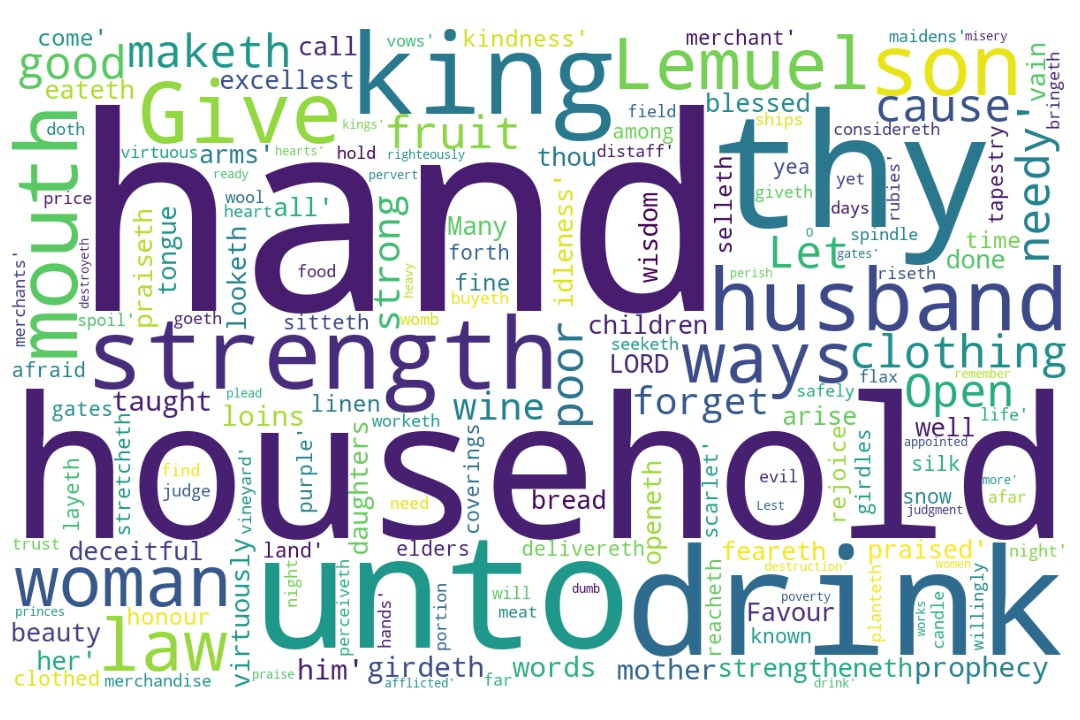
\includegraphics[width=\linewidth]{20OT-Proverbs/Proverb31-WordCloud.jpg}
  \caption{Proverb 31 Word Cloud}
  \label{fig:Proverb 31 word Cloud}
\end{figure}


\marginpar{\scriptsize \centering \fcolorbox{bone}{lime}{\textbf{A DIFFERENT SORT OF WOMAN}}\\ (Proverb 31:1-31) \begin{compactenum}[I.][8]
    \item \textbf{Worth} \index[scripture]{Proverbs!Pro 31:10}(Pro 31:10)
    \item \textbf{Work} \index[scripture]{Proverbs!Pro 31:13}(Pro 31:13)
    \item \textbf{Window} \index[scripture]{Proverbs!Pro 31:18}(Pro 31:18) -- she sets a candle, and her place is known as a sanctuary
    \item \textbf{Wardrobe} \index[scripture]{Proverbs!Pro 31:22}(Pro 31:22) -- not dressed for show, but to be about business
    \item \textbf{Words} \index[scripture]{Proverbs!Pro 31:26}(Pro 31:26)
    \item \textbf{Wisdom} \index[scripture]{Proverbs!Pro 31:26}(Pro 31:26)
    \item \textbf{Wholesomeness} \index[scripture]{Proverbs!Pro 31:30}(Pro 31:30)
\end{compactenum}}

\marginpar{\scriptsize \centering \fcolorbox{bone}{yellow}{\textbf{VIEWING VIRTUE}}\\ (Proverb 31:1-31) \begin{compactenum}[I.][8]
    \item \textbf{Her Purity}\index[scripture]{Proverbs!Pro 31:11} (Pro 31:11) 
    \item \textbf{Her Prudence} 
	\item \textbf{Her Perception} \index[scripture]{Proverbs!Pro 31:19} (Pro 31:19) 
    \item \textbf{Her Patience} \index[scripture]{Proverbs!Pro 31:19} (Pro 31:19) 
    \item \textbf{Her Praiseworthiness} \index[scripture]{Proverbs!Pro 31:28} (Pro 31:28) 
    \item \textbf{Her Productivity} \index[scripture]{Proverbs!Pro 31:15, 19} (Pro 31:15, 19) 
    \item \textbf{Her Pricelessness} \index[scripture]{Proverbs!Pro 31:28} (Pro 31:28)  
\end{compactenum}}

\marginpar{\scriptsize \centering \fcolorbox{bone}{black}{\textbf{\textcolor[cmyk]{0,0,0,0}{LOOK AT THIS ONE!}}}\\ (Proverb 31) \begin{compactenum}[I.][8]
	\item Her \textbf{Price} \index[scripture]{Proverbs!Pro 31:10} (Pro 31:10)
	\item \textbf{Provides} for Others\index[scripture]{Proverbs!Pro 31:15} (Pro 31:15)
	\item Cares for the \textbf{Poor}\index[scripture]{Proverbs!Pro 31:19} (Pro 31:19)
	\item Has Uncanny \textbf{Perception}\index[scripture]{Proverbs!Pro 31:18} (Pro 31:18)
	\item All about \textbf{Prepartion}\index[scripture]{Proverbs!Pro 31:19} (Pro 31:19)
	\item Cares for the \textbf{Poor}\index[scripture]{Proverbs!Pro 31:19} (Pro 31:19)
	\item Her \textbf{Priority} \index[scripture]{Proverbs!Pro 31:27-28} (Pro 31:27-28)
	\item Worth every  \textbf{Praise} \index[scripture]{Proverbs!Pro 31:27-28} (Pro 31:27-28)
\end{compactenum}}

\marginpar{\scriptsize \centering \fcolorbox{bone}{blue}{\textbf{\textcolor[cmyk]{0,0,0,0}{THE HUSBAND OF A}}} \fcolorbox{bone}{blue}{\textbf{\textcolor[cmyk]{0,0,0,0}{VIRTUOUS WOMAN}}}\\ (Proverb 31) 
\begin{compactenum}
    \item \textbf{Treasures Her} \index[scripture]{Proverbs!Pro 31:24}(Pro 31:10)
    \item \textbf{Trusts in Her} \index[scripture]{Proverbs!Pro 31:11}(Pro 31:11)
    \item \textbf{Trades by Her} \index[scripture]{Proverbs!Pro 31:14, 24}(Pro 31:14, 24) 
    \item \textbf{Is Taken Care of by Her} \index[scripture]{Proverbs!Pro 31:12,15,21,27}(Pro 31:12, 15, 21, 27) 
    \item \textbf{Triumphs Because of Her} \index[scripture]{Proverbs!Pro 31:23}(Pro 31:23) 
    \item \textbf{Thanks Her} \index[scripture]{Proverbs!Pro 31:28, 30}(Pro 31:28, 30) 
    \item \textbf{He Entrusts Her} The husband of a virtuous woman will entrust her with resources.  She will not be extravagant. She will not be foolish. Instead she will use the resources wisely to be a blessing to her family or others. \index[scripture]{Proverbs!Pro 31:28, 30}(Pro 31:28,30)
\end{compactenum}}

\footnote{\textcolor[cmyk]{0.99998,1,0,0}{\hyperlink{TOC}{Return to end of Table of Contents.}}}\footnote{\href{https://www.audioverse.org/english/audiobibles/books/ENGKJV/O/Prov/1}{\textcolor[cmyk]{0.99998,1,0,0}{Proverbs Audio}}}\textcolor[cmyk]{0.99998,1,0,0}{The words of king Lemuel, the prophecy that his mother taught him.}
[2] \textcolor[cmyk]{0.99998,1,0,0}{What, my son? and what, the son of my womb? and what, the son of my vows?}
[3] \textcolor[cmyk]{0.99998,1,0,0}{Give not thy strength unto women, nor thy ways to that which destroyeth kings.}
[4] \textcolor[cmyk]{0.99998,1,0,0}{\emph{It} \emph{is} not for kings, O Lemuel, \emph{it} \emph{is} not for kings to drink wine; nor for princes strong drink:}
[5] \textcolor[cmyk]{0.99998,1,0,0}{Lest they drink, and forget the law, and pervert the judgment of any of the afflicted.}
[6] \textcolor[cmyk]{0.99998,1,0,0}{Give strong drink unto him that is ready to perish, and wine unto those that be of heavy hearts.}
[7] \textcolor[cmyk]{0.99998,1,0,0}{Let him drink, and forget his poverty, and remember his misery no more.}
[8] \textcolor[cmyk]{0.99998,1,0,0}{Open thy mouth for the dumb in the cause of all such as are appointed to destruction.}
[9] \textcolor[cmyk]{0.99998,1,0,0}{Open thy mouth, judge righteously, and plead the cause of the poor and needy.}
[10] \textcolor[cmyk]{0.99998,1,0,0}{Who can find a virtuous woman? for her price \emph{is} far \fcolorbox{bone}{lime}{above rubies}.}
[11] \textcolor[cmyk]{0.99998,1,0,0}{The heart of her husband doth safely trust in her, so that he shall have no need of spoil.}
[12] \textcolor[cmyk]{0.99998,1,0,0}{She will do him good and not evil all the days of her life.}
[13] \textcolor[cmyk]{0.99998,1,0,0}{She seeketh wool, and flax, and \fcolorbox{bone}{lime}{worketh} willingly with her hands.}
[14] \textcolor[cmyk]{0.99998,1,0,0}{She is like the merchants' ships; she bringeth her food from afar.}
[15] \textcolor[cmyk]{0.99998,1,0,0}{She riseth also while it is yet night, and giveth meat to her household, and a portion to her maidens.}
[16] \textcolor[cmyk]{0.99998,1,0,0}{She considereth a field, and buyeth it: with the fruit of her hands she planteth a vineyard.}
[17] \textcolor[cmyk]{0.99998,1,0,0}{She girdeth her loins with strength, and \fcolorbox{bone}{MYGOLD}{strengtheneth} her arms.}
[18] \textcolor[cmyk]{0.99998,1,0,0}{She perceiveth that her merchandise \emph{is} good: her \fcolorbox{bone}{lime}{candle} goeth not out by night.}
[19] \textcolor[cmyk]{0.99998,1,0,0}{She layeth her hands to the spindle, and her hands hold the distaff.}
[20] \textcolor[cmyk]{0.99998,1,0,0}{She stretcheth out her hand to the poor; yea, she reacheth forth her hands to the needy.}
[21] \textcolor[cmyk]{0.99998,1,0,0}{She is not afraid of the snow for her household: for all her household \emph{are} clothed with scarlet.}
[22] \textcolor[cmyk]{0.99998,1,0,0}{She maketh herself coverings of \fcolorbox{bone}{lime}{tapestry}; her clothing \emph{is} silk and purple.}
[23] \textcolor[cmyk]{0.99998,1,0,0}{Her husband is known in the gates, when he sitteth among the elders of the land.}
[24] \textcolor[cmyk]{0.99998,1,0,0}{She maketh fine linen, and selleth \emph{it}; and delivereth girdles unto the merchant.}
[25] \textcolor[cmyk]{0.99998,1,0,0}{Strength and honour \emph{are} her clothing; and she shall rejoice in time to come.}
[26] \textcolor[cmyk]{0.99998,1,0,0}{She openeth her \fcolorbox{bone}{lime}{mouth} with \fcolorbox{bone}{lime}{wisdom}; and in her \fcolorbox{bone}{lime}{tongue} \emph{is} the law of kindness.}
[27] \textcolor[cmyk]{0.99998,1,0,0}{She looketh well to the ways of her household, and eateth not the bread of idleness.}
[28] \textcolor[cmyk]{0.99998,1,0,0}{Her children arise up, and call her blessed; her husband \emph{also}, and he praiseth her.}
[29] \textcolor[cmyk]{0.99998,1,0,0}{Many daughters have done virtuously, but thou excellest them all.}
[30] \textcolor[cmyk]{0.99998,1,0,0}{Favour \emph{is} deceitful, and beauty \emph{is} vain: \emph{but} a woman \emph{that} feareth the LORD, she shall be \fcolorbox{bone}{lime}{praised}.}
[31] \textcolor[cmyk]{0.99998,1,0,0}{Give her of the fruit of her hands; and let her own works praise her in the gates.}



